% ============================================================
% Progress-meeting slide deck — compiles as-is on Overleaf (pdfLaTeX).
% No external images required; only standard packages (beamer, tikz,
% booktabs, amsmath/amssymb, array, textcomp).
% ============================================================

\documentclass[aspectratio=169]{beamer}

\usetheme{Madrid}
\usecolortheme{default}
\setbeamertemplate{navigation symbols}{}
\setbeamertemplate{footline}[frame number]
\setbeamercolor{block title}{bg=blue!20,fg=black}
\setbeamercolor{block body}{bg=blue!5,fg=black}

\usepackage[utf8]{inputenc}
\usepackage{textcomp}
\usepackage{amsmath}
\usepackage{amssymb}
\usepackage{booktabs}
\usepackage{array}
\usepackage{tikz}
\usetikzlibrary{arrows.meta,positioning}

\renewcommand{\arraystretch}{0.95}

\title[UAV 360\textdegree\ Streaming RL]{UAV-Assisted Tile-Selective 360\textdegree\ Video Streaming}
\subtitle{Reinforcement Learning Environment --- Progress Summary}
\author{Jad Al Lakkis}
\date{\today}

\begin{document}

\begin{frame}
  \titlepage
\end{frame}

\begin{frame}{Outline}
  \tableofcontents
\end{frame}

\section{Problem Formulation}

\begin{frame}{Constrained MDP: Objective \& Constraints}
  \framesubtitle{Tile-selective enhancement for UAV-served 360\textdegree\ video}

  \begin{block}{Objective (eq.\ 5)}
    \[ \max \; \mathbb{E}\Big[\textstyle\sum_t \lambda^t \, \bar Q^t_{\text{viewport}}\Big], \qquad \lambda = 0.01 \]
  \end{block}

  \begin{block}{Subject to long-run budget constraints (eqs.\ 6--8)}
    \begin{itemize}
      \item $\mathbb{E}[D^t] \le \bar D$ \quad --- stall-time budget
      \item $\mathbb{E}[P^t] \le \bar P$ \quad --- transmit-power budget
      \item $\mathbb{E}[B^t] \le \bar B$, \ $B^t = \frac{1}{N}\sum_i x_i^t$ \quad --- enhanced-tile-fraction budget
    \end{itemize}
  \end{block}

  \vspace{2pt}
  Decision each slot $t$: which of $N{=}64$ tiles to enhance, and at what transmit power.
\end{frame}

\begin{frame}{Per-Step Training Reward (eq.\ 9)}
  \[ r^t \;=\; \beta_Q\,\bar Q^t_{\text{viewport}} \;-\; \beta_S\,\frac{D^t}{T_0} \;-\; \beta_P\,\frac{P^t}{P_{\max}} \;-\; \beta_B\,\frac{1}{N}\sum_i x_i^t \]

  \begin{itemize}
    \item One term per constraint: quality reward, stall penalty, power penalty, tile-budget penalty
    \item Currently $\beta_Q=\beta_S=\beta_P=\beta_B=1.0$ --- equal weights, a placeholder (open question)
    \item This penalty reward is what the environment trains against today; it is a \emph{soft} stand-in for the constraints above, not an enforcement mechanism --- see ``Lagrangian'' later
  \end{itemize}
\end{frame}

\section{Implementation}

\begin{frame}{Professor's Feedback $\to$ \texttt{config.py}}
  \begin{center}
  \footnotesize
  \begin{tabular}{@{}>{\raggedright\arraybackslash}p{0.24\linewidth}>{\raggedright\arraybackslash}p{0.68\linewidth}@{}}
    \toprule
    \textbf{Point raised} & \textbf{Resolved into \texttt{config.py}} \\
    \midrule
    Channel model & Reuse MMSP'25 Rician + path-loss as-is: $P_{\max}{=}20$dBm, $W{=}10$MHz, $T_0{=}1$s, $N_0{=}{-}174$dBm/Hz, $K{=}12$dB \\
    Base/enhancement layers & Highest QP = base layer, $k$ extra layers = enhancement. Array index $= 6-k$. Cross-checked: $A_{\text{base}}\approx4.41$Mbps vs.\ paper's $\approx4.5$Mb \\
    FOV / mobility / video & $V_\theta{=}60^\circ$, $V_\phi{=}30^\circ$; static distance $d{=}50$m; train on \texttt{Runner} first \\
    Constraint budgets & $\bar B\approx0.20$ (9--16 tiles, geometric); $\bar P$, $\bar D$ still open --- no UAV spec / sweep values yet \\
    \bottomrule
  \end{tabular}
  \end{center}

  \vspace{4pt}
  \scriptsize
  \begin{itemize}
    \item Also resolved this session: area-weighted partial-tile visibility
    \item 1-critic baseline $\to$ 2 critics once post-decision states are added
    \item Yaw/pitch/roll range \& units confirmed empirically from 194 real traces
  \end{itemize}
\end{frame}

\begin{frame}{The Environment: \texttt{TileStreamingEnv}}
  \begin{center}
  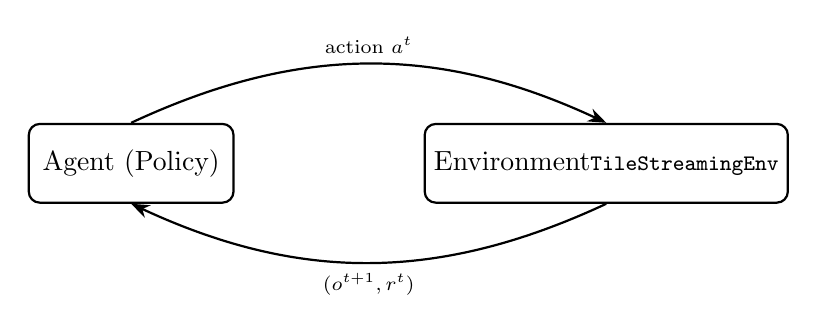
\begin{tikzpicture}[node distance=2.4cm, >=Stealth, thick]
    \node[draw, rounded corners, minimum width=2.6cm, minimum height=1cm] (agent) {Agent (Policy)};
    \node[draw, rounded corners, minimum width=3.4cm, minimum height=1cm, right=of agent] (env) {Environment\\ \footnotesize\texttt{TileStreamingEnv}};
    \draw[->] (agent.north) to[bend left=25] node[above,font=\scriptsize]{action $a^t$} (env.north);
    \draw[->] (env.south) to[bend left=25] node[below,font=\scriptsize]{$(o^{t+1}, r^t)$} (agent.south);
  \end{tikzpicture}
  \end{center}

  \begin{itemize}
    \item Standard \texttt{gymnasium.Env} --- plugs directly into \texttt{stable-baselines3}
    \item Observation $o^t = (Z^t, \Delta\theta^t, \Delta\phi^t, h^t)$: buffer level, viewport-prediction error, channel gain
    \item Action $a^t$: 64 binary tile-enhance flags + 1 of 5 discrete power levels (flat \texttt{MultiDiscrete})
    \item One episode = one real head-trace; \texttt{Runner} gives 36 decision steps (1080 frames / 30 frames-per-GOP)
  \end{itemize}
\end{frame}

\begin{frame}{What \texttt{step()} Actually Computes}
  \begin{enumerate}
    \item Unpack action $\to$ tile mask $x^t$, transmit power $P^t$
    \item Compute data volume $A^t$, rate $R^t$ (Shannon capacity via $h^t$), stall $D^t$, next buffer $Z^{t+1}$
    \item Reveal the real recorded viewport for slot $t$; compute area-weighted coverage $\bar Q^t$ and prediction error $(\Delta\theta^t,\Delta\phi^t)$
    \item Reward $r^t = r_{\text{known}} + r_{\text{random}}$ (penalty terms + coverage term)
    \item Sample next channel gain $h^{t+1}$; return the next observation
  \end{enumerate}

  \vspace{6pt}
  \texttt{reset()}: picks a random valid trace, sets $Z^0{=}0$, and bootstraps the first prediction to the true position (zero initial error by construction).
\end{frame}

\begin{frame}{Channel Model: Rician Fading + Path Loss}
  \[ h^t = \frac{3.24\times10^{-4}\,|\psi^t|^2}{\left(d\cdot\tan^{-1}\!\left(\frac{24\sqrt2}{5}\right)\right)^2} \]
  \[ R^t = W\log_2\!\left(1+\frac{P^t h^t}{N_0 W}\right) \]

  \begin{itemize}
    \item $\psi^t$: Rician fading, $K{=}12$dB, $\mathbb{E}[|\psi^t|^2]{=}1$
    \item Real \& imaginary parts of $\psi^t$ drawn independently from matched Normal distributions --- implemented literally per the paper's stated form
    \item $d{=}50$m, fixed (static UAV distance, per professor's guidance)
    \item Adopted directly from the related MMSP'25 channel model
  \end{itemize}
\end{frame}

\begin{frame}{Codebase Structure}
  \scriptsize
  \begin{tabular}{@{}>{\raggedright\arraybackslash}p{0.30\linewidth}>{\raggedright\arraybackslash}p{0.64\linewidth}@{}}
    \toprule
    \textbf{File} & \textbf{Purpose} \\
    \midrule
    \texttt{config.py} & Single source of truth for every parameter and convention \\
    \texttt{data\_loader.py} & Loads the dataset: video catalog, \texttt{hn.mat}/\texttt{rd.mat}, valid-trace classification \\
    \texttt{channel\_model.py} & Rician fading + path loss $\to$ channel gain; Shannon rate \\
    \texttt{layer\_model.py} & $A^t = A_{\text{base}} + \sum_i x_i^t \Delta A_i^t$ --- data volume per slot \\
    \texttt{viewport.py} & Yaw/pitch $\to$ viewport rectangle $\to$ per-tile area-weighted coverage \\
    \texttt{environment.py} & \texttt{TileStreamingEnv} --- the gymnasium \texttt{Env} itself \\
    \texttt{sanity\_check.py} & Runs random-policy episodes, checks for numerically sane behavior \\
    \texttt{tests/test\_channel\_model.py} & Empirical statistical checks on the channel model \\
    \bottomrule
  \end{tabular}
\end{frame}

\section{Verification}

\begin{frame}{Verification --- What Was Actually Tested}
  \scriptsize
  \begin{tabular}{@{}>{\raggedright\arraybackslash}p{0.34\linewidth}>{\raggedright\arraybackslash}p{0.60\linewidth}@{}}
    \toprule
    \textbf{Component} & \textbf{Result} \\
    \midrule
    Channel model (500k samples) & $\mathbb{E}[|\psi|^2]=0.99972$ (target 1.0); LOS/scatter ratio $=15.858$ (target $\nu=15.849$) \\
    Channel model (10k samples) & All gains finite \& $\ge0$; seeded runs bit-identical, different seeds differ \\
    Layer model (\texttt{Runner}, 0 tiles enhanced) & $A_{\text{base}} = 4{,}411{,}432$ bits ($\approx4.41$Mbps) \\
    Viewport (incl.\ $\pm180^\circ$ wraparound) & Covered area $=$ viewport area (7{,}200 square degrees) exactly, every case tested \\
    Data loader & 15 videos in catalog; 12 valid traces for \texttt{Runner} \\
    Full environment & Passes gymnasium \texttt{check\_env}; 5$\times$36-step random-policy episodes --- zero negative buffer, zero NaN/Inf \\
    \bottomrule
  \end{tabular}
\end{frame}

\section{Status \& Next Steps}

\begin{frame}{Implemented vs.\ Not Yet Implemented}
  \footnotesize
  \begin{columns}[T]
    \begin{column}{0.48\textwidth}
      \textcolor{green!50!black}{\textbf{Implemented \& verified}}
      \begin{itemize}
        \item Full single-agent MDP loop (state, action, reward, transition) as a working Gym env
        \item Real dataset values for video content, not synthetic placeholders
        \item Paper-faithful Rician channel model
      \end{itemize}
    \end{column}
    \begin{column}{0.48\textwidth}
      \textcolor{red!70!black}{\textbf{Not yet implemented}}
      \begin{itemize}
        \item Post-decision states, second critic, virtual experience (phase 2)
        \item Predicted-viewport tiles are not forced to be enhanced
        \item $\bar D,\bar P,\bar B$ not enforced --- only the per-step penalty reward exists
        \item PPO training script (\texttt{torch} install in progress)
      \end{itemize}
    \end{column}
  \end{columns}
\end{frame}

\begin{frame}{Constraint Enforcement: Lagrangian Relaxation}
  \begin{alertblock}{Next step}
    Implement Lagrangian / primal-dual relaxation so $\bar D,\bar P,\bar B$ are actually \emph{enforced}, not just softly discouraged by fixed reward weights.
  \end{alertblock}

  \vspace{4pt}
  One multiplier per constraint, $\mu_D,\mu_P,\mu_B \ge 0$:
  \begin{align*}
    \mathcal{L} \;=\;& \mathbb{E}\Big[\textstyle\sum_t\lambda^t \bar Q^t\Big] \\
    & - \mu_D\big(\mathbb{E}[D^t]-\bar D\big) - \mu_P\big(\mathbb{E}[P^t]-\bar P\big) - \mu_B\big(\mathbb{E}[B^t]-\bar B\big)
  \end{align*}

  \begin{itemize}
    \item Multipliers updated via dual gradient ascent, based on observed constraint violation --- alongside the usual policy update
    \item Mathematically equivalent to the original CMDP (eqs.\ 5--8) --- a more rigorous solution method, not a redefinition of the problem
  \end{itemize}
\end{frame}

\begin{frame}{Open Questions for the Meeting}
  \footnotesize
  \begin{columns}[T]
    \begin{column}{0.48\textwidth}
      \begin{itemize}
        \item Enhancement level $k$: which value?
        \item Force-enhance predicted-viewport tiles, or leave the agent fully free?
        \item Selected tile sent whole at enhanced quality, or partial-tile transmission?
        \item Initial buffer $Z^0$: empty, or pre-buffered?
        \item $\bar P$: real UAV/battery number?
      \end{itemize}
    \end{column}
    \begin{column}{0.48\textwidth}
      \begin{itemize}
        \item $\bar D$: which candidate values to sweep?
        \item Is the per-step penalty enough for now, or is Lagrangian needed immediately?
        \item Reward weights $\beta_Q,\beta_S,\beta_P,\beta_B$: equal, or prioritized?
        \item Tile-index $\to$ grid-position order: confirmed raster order?
        \item Yaw positive direction, observation scaling: confirm conventions?
      \end{itemize}
    \end{column}
  \end{columns}
\end{frame}

\begin{frame}{Next Steps}
  \begin{enumerate}
    \item Resolve the open questions above with the professor
    \item Decide \& implement constraint enforcement (Lagrangian) and the predicted-viewport policy
    \item Finish installing \texttt{torch} (CPU) + \texttt{stable-baselines3}
    \item Build \texttt{train\_ppo.py}; train a first PPO baseline
    \item Validate the baseline against a simple reference policy
    \item Add post-decision states, second critic, virtual experience (phase 2)
    \item Longer-term: multi-video training, full UAV mobility modeling
  \end{enumerate}
\end{frame}

\begin{frame}
  \centering
  \vspace{2cm}
  {\Huge Thank You}\\[1em]
  {\large Questions?}
\end{frame}

\end{document}
